%%%%%%%%%%%%%%%%%%%%%%%%%%%%%%%%%%%%%%%%%
% baposter Portrait Poster
% LaTeX Template
% Version 1.0 (15/5/13)
%
% Created by:
% Brian Amberg (baposter@brian-amberg.de)
%
% This template has been downloaded from:
% http://www.LaTeXTemplates.com
%
% License:
% CC BY-NC-SA 3.0 (http://creativecommons.org/licenses/by-nc-sa/3.0/)
%
%%%%%%%%%%%%%%%%%%%%%%%%%%%%%%%%%%%%%%%%%

%-------------------------------------------------------------------------------
%---------
%	PACKAGES AND OTHER DOCUMENT CONFIGURATIONS
%-------------------------------------------------------------------------------
%---------

\documentclass[a0paper,landscape]{baposter}

% Required for specifying captions to tables and figures
\usepackage[font=small,labelfont=bf]{caption} 
\usepackage{booktabs} % Horizontal rules in tables
\usepackage{relsize} % Used for making text smaller in some places
\usepackage{textcomp}
\usepackage{amsmath}  %Nécessaire pour les maths 
\usepackage{amssymb}  %Nécessaire pour les maths 

\graphicspath{{../resources/pictures}} % Directory in which figures are stored

\definecolor{bordercol}{RGB}{40,40,40} % Border color of content boxes
% Background color for the header in the content boxes (left side)
\definecolor{headercol1}{RGB}{186,215,230}
% Background color for the header in the content boxes (right side)
\definecolor{headercol2}{RGB}{80,80,80}
% Text color for the header text in the content boxes
\definecolor{headerfontcol}{RGB}{0,0,0}
% Background color for the content in the content boxes
\definecolor{boxcolor}{RGB}{255, 255, 255}

\newcommand{\hmm}{\textsc{HMM}}
\newcommand{\mcmc}{\textsc{MCMC}}
\newcommand{\fhmm}{\textsc{Factorial HMM}}
\newcommand{\Estep}{\textsc{E-step}}
\newcommand{\Mstep}{\textsc{M-step}}
\newcommand{\EM}{\textsc{EM}}
\newcommand{\meanfield}{\textsc{mean-field}}
\newcommand{\structmeanfield}{\textsc{structured mean-field}}

\begin{document}

\background{ % Set the background to an image (background.pdf)
\begin{tikzpicture}[remember picture,overlay]
% \draw (current page.north west)+(-2em,2em) node[anchor=north west]
% {\includegraphics[height=1.1\textheight]{background}};
\end{tikzpicture}
}

\begin{poster}{
grid=false,
borderColor=bordercol, % Border color of content boxes
% Background color for the header in the content boxes (left side)
headerColorOne=headercol1,
% Background color for the header in the content boxes (right side)
headerColorTwo=headercol2,
% Text color for the header text in the content boxes
headerFontColor=headerfontcol,
% Background color for the content in the content boxes
boxColorOne=boxcolor,
% Specify the rounded corner in the content box headers
headershape=roundedright,
% Font modifiers for the text in the content box headers
headerfont=\Large\sf\bf,
textborder=rectangle,
background=user,
headerborder=open, % Change to closed for a line under the content box headers
boxshade=plain
}
{}
%
%----------------------------------------------------------------------------------------
%	TITLE AND AUTHOR NAME
%----------------------------------------------------------------------------------------
%
{\sf\bf Factorial HMM} % Poster title
{Th\'{e}is Bazin, Valentin De Bortoli, \'{E}lie Michel\\ % Author names
% Author email addresses
{\smaller \textlangle{} theis.bazin, vdeborto, elie.michel \textrangle{} @ ens-paris-saclay.fr}}
{
\includegraphics[scale=0.2]{../resources/pictures/logos/logo-ens_paris_saclay.png}} % University/lab logo

%----------------------------------------------------------------------------------------
%	INTRODUCTION
%----------------------------------------------------------------------------------------

\headerbox{Introduction}{name=introduction,column=0,row=0}{

We present the Factorial Hidden Markov Model, \fhmm{}, as introduced by
Ghahramani and Jordan, an extension of \hmm{}, and methods to
perform inference on this model.

\begin{description}
 \item[Context] \hmm{} assumes the hidden variable to be single multinomial variable,
 this can lead to computational issues,
 \item[HMM limitation] Suppose we want to describe $M=30$ binary states~\cite{ghahramani1997factorial},
    \begin{itemize}
      \item Using \hmm{} the state space has size $2^{30}$,
      \item Using \textit{distributed} reduces this to only $M=30$ binary states.
    \end{itemize}
\end{description}


This yields the \fhmm{} model.

\begin{center}
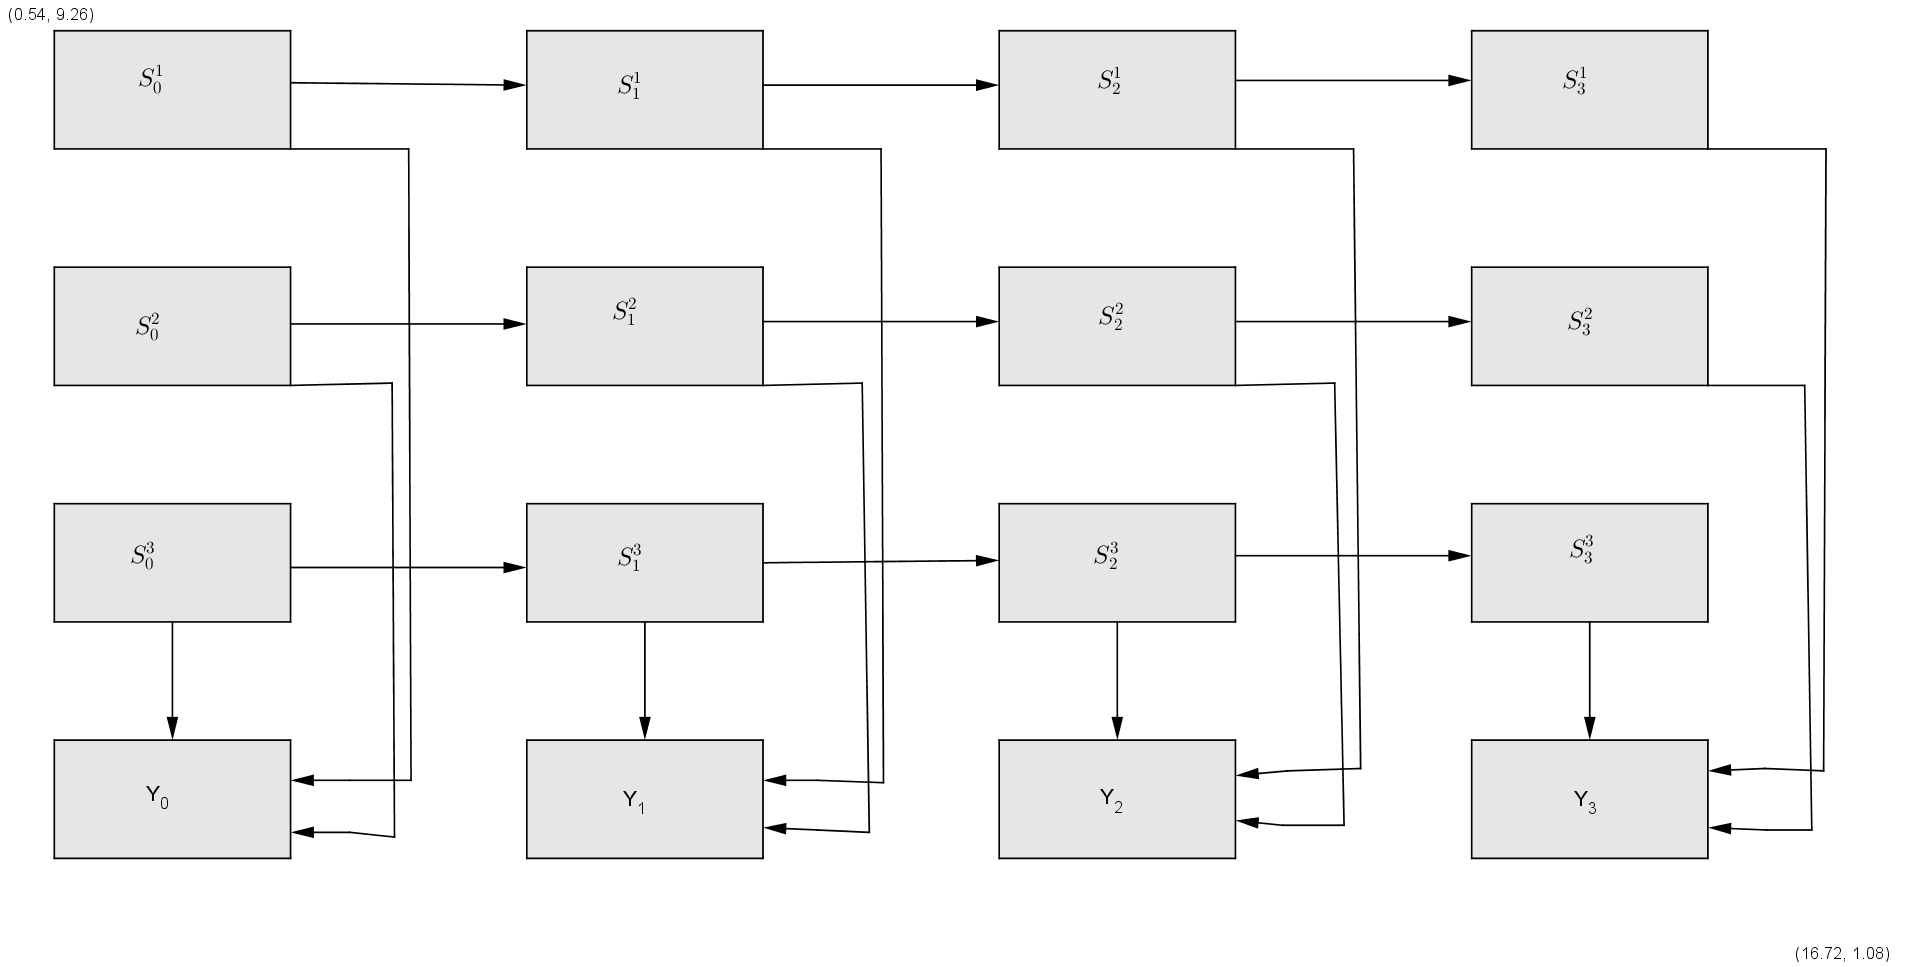
\includegraphics[width=0.8\linewidth]{../resources/pictures/facthmm.png}
\captionof{figure}{Graphical model for Factorial HMM}
\end{center}
}

%----------------------------------------------------------------------------------------
%	AN EM ALGORTIHM...
%----------------------------------------------------------------------------------------

\headerbox{An EM algorithm...}{name=methods,column=0,below=introduction,above=bottom}{
Training this model can be done per the \EM{} algorithm \cite{wu1983convergence}.
\begin{description}
  \item[\Estep{}] Compute the posterior $p(S_{(t)}^{(m)} \vert Y_{(t)}, \theta)$
  \item[\Mstep{}] Update the parameters $\theta$
\end{description}
\Mstep{} is \emph{easy} but \Estep{} can be
\emph{really hard}~\cite{ghahramani1997factorial} to compute.
Recall that in the \hmm{} we used an alpha-beta recursion to deal with the
\Estep{}.

We present three different ways to deal with \Estep{}:
\begin{itemize}
  \item Exact inference,
  \item Gibbs sampling,
  \item Variational methods.
\end{itemize}
}

%----------------------------------------------------------------------------
%	Exact inference
%----------------------------------------------------------------------------

\headerbox{Exact inference}{name=exactinference,column=1,row=0}{

The exact inference allows us to compute the posterior distribution setting:
\begin{equation}
\left\lbrace
\begin{aligned}
&\alpha_t = p(S_t^1, \dots, S_t^M, Y_{(1,t)} \vert \theta)\\
&\alpha_t^m = p(S_{t-1}^1,\dots,S_{t-1}^m,S_t^{m+1},\dots,S_t^M \vert \theta)\\
&\beta_t = p(Y_{t+1,T} \vert S_t^1, \dots, S_t^M, \theta) \\
&\beta_{t-1}^m = p(Y_{t+1,T} \vert S_t^1,\dots,S_t^m,S_{t-1}^{m+1},\dots,S_{t-1}^M, \theta)
\end{aligned}
\right.
\end{equation}
Thus we have:
\begin{equation}
\gamma_t = P(S_t \vert Y_{(t)}, \theta) \propto \alpha_t \beta_t
\end{equation}
$\alpha_t$ and $\beta_t$ can be computed recursively:\\
GRAPH
}

%----------------------------------------------------------------------------
%	Gibbs sampling
%----------------------------------------------------------------------------

\headerbox{Gibbs sampling}{name=gibbs,span=1,column=1,below=exactinference}{
% To reduce this block to 1 column width, remove 'span=2'

To go through we do not need to compute the posterior but only
$\langle S_t^m \rangle$, $\langle S_t^m S_t^n \rangle$ and
$\langle S_{t-1}^m S_t \rangle$.
Using the law of large numbers and \mcmc{} methods we can avoid doing exact
inference.
We use Gibbs sampling here.
Since we have a graph structure the iteration gives:
\begin{equation}
\begin{aligned}
&P(S_{t}^m \vert S_{(-t)}^{(m)}, Y_{(t)},\theta) \propto \\ &P(S_t^m \vert S_{t-1}^m)P(S_{t+1}^m \vert S_t^m)P(Y_t \vert S_t^{(m)})
\end{aligned}
\end{equation}

We use an "impatient" Gibbs sampler, i.e no burn-in samples and only a few.\\
We do not try to reach convergence since this algorithm can be very slow.
}

%----------------------------------------------------------------------------
%	RESULTS
%----------------------------------------------------------------------------

\headerbox{Results}{name=results,column=2,span=2,row=0}{
We implemented all the four described methods and tested our implementation
computing the evolution of the log-likelihood (experiments: $K=2$, $M=3)$.

\begin{center}
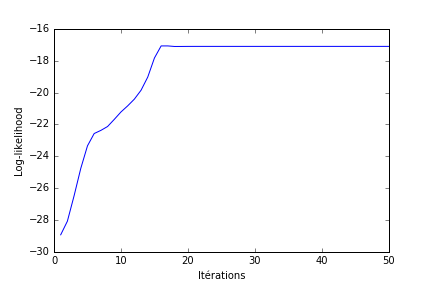
\includegraphics[width=0.17\linewidth]{../resources/pictures/M3_K2_fhmm_exact.png}
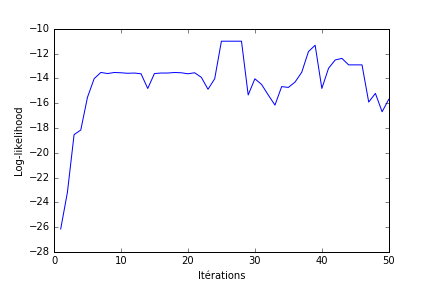
\includegraphics[width=0.17\linewidth]{../resources/pictures/M3_K2_gibbsnoburning.png}
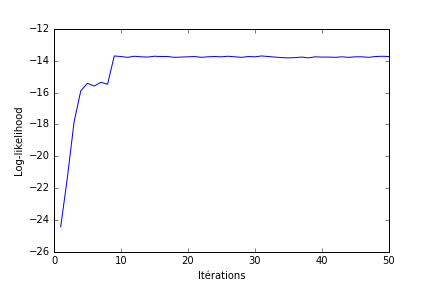
\includegraphics[width=0.17\linewidth]{../resources/pictures/M3_K2_gibbs.png}
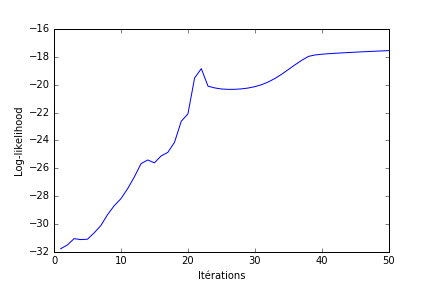
\includegraphics[width=0.17\linewidth]{../resources/pictures/M3_K2_meanfield.png}
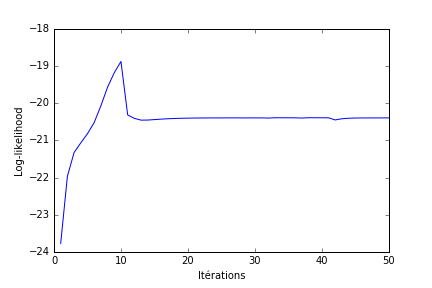
\includegraphics[width=0.17\linewidth]{../resources/pictures/M3_K2_structmeanfield.png}
\captionof{figure}{Log-likelihood over EM iterations for the different models
  (from left to right: exact inference, impatient Gibbs sampling, Gibss
  sampling with burn-in, mean-field, structured mean-field)}
\end{center}

Note that the log-likelihood is not always increasing for the variational
models since we compute an approximated log-likelihood.

In \cite{ghahramani1997factorial} the author suggested using only 10 samples
and no burn-in for the Gibbs sampling however we found that adding a small
burn-in period smoothed our log-likelihood.

\begin{center}
\small
\begin{tabular}{|c|c|}
\hline
\Estep{} method & Iteration duration (s) \\
\hline \hline
\hmm - exact inference & 0.453  \\ \hline
\fhmm - exact inference & 0.429 \\ \hline
Gibbs sampling &  1.100 \\ \hline
\meanfield & 0.053 \\ \hline
\structmeanfield & 0.319 \\ \hline
\end{tabular}
\captionof{table}{Computation times}
\end{center}
% \newline

As $M$ increases exact inference became intractable and Gibbs sampling inefficient.
Variational methods are still satisfactory though.}

%----------------------------------------------------------------------------
%	VARIATIONAL METHODS
%----------------------------------------------------------------------------

\headerbox{Variational methods}{name=variational,column=2,span=1,below=results,
above=bottom}{
Using \mcmc{} we have no information regarding the speed of convergence to the
posterior. 

We now introduce a new family of methods which put constraints on the \Estep{}
thus not yielding the posterior but a \textit{constrained} posterior:
\begin{itemize}
\item \meanfield{}: all hidden states are supposed independent,
\item \structmeanfield{}: we relax the constraint and suppose we have $M$
  independent Markov chains.
\end{itemize}

\begin{center}
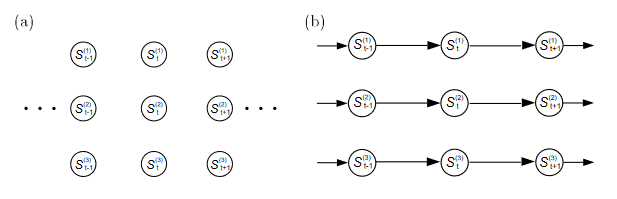
\includegraphics[width=0.6\linewidth]{../resources/pictures/gm_variational.png}
\captionof{figure}{Graphical models for the variational inference
(from left to right: mean-field, structure mean-field)}
\end{center}

% The distance between the true posterior and this approximate proability is
% % given by $\text{KL}(q \| p(S_{(t)}^{(m)} \vert Y_{(t)}, \theta)$ where KL is
% computed via the Kullback-Leiber divergence.
% We iteratively minimize this quantity.
}

%----------------------------------------------------------------------------------------
%	CONCLUSION & FUTURE WORK
%----------------------------------------------------------------------------------------

\headerbox{Conclusion and future work...}{name=conclusion,column=3,span=1,below=results,
above=bottom}{
In our work:
\begin{itemize}
 \item We implemented the four methods to perform inference (the \Estep{}) on
 \fhmm{},
 \item we investigated the mathematical model behind \fhmm{},
 \item and we experimentally verified the benefits of variationnal models in
 dealing with large space states.
\end{itemize}

\begin{description}
 \item[What's next] As next steps, we wish to test our implementation on real
 data (the Bach Chorales) and compare the properties of this model versus
 \hmm{} on test data.
\end{description}

}

%----------------------------------------------------------------------------------------

%----------------------------------------------------------------------------------------
%	REFERENCES
%----------------------------------------------------------------------------------------

\headerbox{References}{name=conclusion,column=1,span=1,below=gibbs,above=bottom}{
% \smaller % Reduce the font size in this block
\renewcommand{\section}[2]{\vskip 0.05em} % Get rid of the default "References" section title
\nocite{*} % Insert publications even if they are not cited in the poster


\bibliographystyle{plain}
\bibliography{../resources/bibliography/bibfile}\
}

%----------------------------------------------------------------------------------------
\end{poster}

\end{document}\grid
